\documentclass[./main.tex]{subfiles}
\graphicspath{{\subfix{./figs}}}

% ------------ main document ------------
\begin{document}
\nolinenumbers

% style setup
\newpage
\renewcommand{\headrulewidth}{0pt}
\thispagestyle{fancy}
%... then configure it
\fancyhf{} % Clear all header and footer fields.
\fancyfoot{} % clear all footer fields
\fancyfoot[C]{\thepage}

\par \hfill
\vspace{40mm}
\begin{adjustwidth}{45pt}{45pt}
\begin{center}
    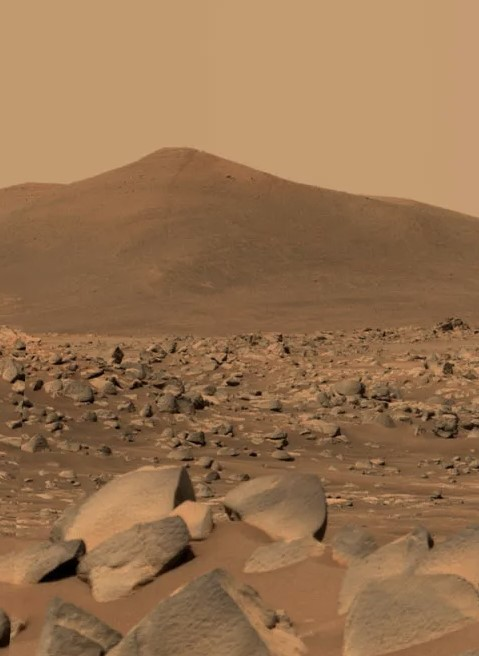
\includegraphics[scale=0.7]{figs/mars.jpg}\\
\end{center}
\vspace{10mm}
\noindent \textsf{Marte possui um terreno rochoso e arenoso. A atmosfera é composta por aproximadamente 95\% de dióxido de carbono, com uma pressão atmosférica média de cerca de 600 Pa. As temperaturas variam drasticamente, com médias em torno de -60°C. O planeta não possui corpos d'água em estado líquido, e sua superfície é constantemente exposta à radiação cósmica e solar devido à ausência de um campo magnético.}
\end{adjustwidth}
\clearpage
\end{document}